\documentclass[aspectratio=169,9pt]{beamer}

\usetheme{Madrid}
\usecolortheme{seahorse}
\usepackage[utf8]{inputenc}
\usepackage{amsmath}
\usepackage{listings}
\usepackage{xcolor}
\usepackage{graphicx}
\usepackage{booktabs}
\usepackage{tabularx}

\lstdefinestyle{cli}{
  basicstyle=\ttfamily\scriptsize,
  backgroundcolor=\color{black!5},
  frame=single,
  breaklines=true,
  columns=fullflexible,
  keywordstyle=\color{blue},
}
\lstdefinestyle{va}{
  basicstyle=\ttfamily\scriptsize,
  backgroundcolor=\color{black!5},
  frame=single,
  breaklines=true,
  columns=fullflexible,
}
\lstnewenvironment{cli}{\lstset{style=cli}}{}
\lstnewenvironment{va}{\lstset{style=va}}{}

\title{A Real 2x2 Memristor Crossbar}
\subtitle{A full, real design example on openMemristorPDK -- layout, extraction, LVS, DRC, and a real write-then-read simulation with sneak-path disturb}
\author{}
\date{}

\begin{document}

\frame{\titlepage}

% ---------------------------------------------------------------
\begin{frame}{What gets built, and why it's harder than one cell}
\footnotesize
\begin{itemize}
  \item Every earlier deck in this project builds one, isolated
        2-terminal memristor cell. A real crossbar array is
        genuinely different: two or more cells share the same real
        bottom-electrode row and top-electrode column -- the whole
        point of a crossbar (dense, wire-efficient addressing), and
        the whole reason it needs its own real worked example.
  \item Two real design decisions, confirmed before any real work
        started: a genuine shared-row/shared-column topology (not
        four separately-wired single-cell instances), and a real
        write-then-read protocol that makes the classic crossbar
        \textbf{sneak-path disturb} visible, not just a per-cell DC
        sweep.
  \item Every real step below -- layout, LEF, extraction, LVS, DRC,
        simulation -- is the literal, real action taken, including a
        real, found-live tool limitation this exact build ran into
        and had to work around honestly, not hide.
\end{itemize}
\end{frame}

% ---------------------------------------------------------------
\begin{frame}[fragile]{Step 1 -- the real crossbar topology}
Two real bottom-electrode (\texttt{be\_au}) rows, two real
top-electrode (\texttt{te\_au}) columns, real \texttt{mem\_tio2}
oxide only at the 4 real crosspoints where a row and a column
actually overlap:
\begin{center}
\begin{tabularx}{\textwidth}{lX}
\toprule
Element & Real geometry (microns) \\
\midrule
BE1 (row) & $y \in [2,3]$, $x \in [0,9]$ -- 1um wide, spans the full array \\
BE2 (row) & $y \in [6,7]$, $x \in [0,9]$ -- 3um real gap from BE1, well past any real DRC minimum \\
TE1 (column) & $x \in [2,3]$, $y \in [0,9]$ -- 1um wide, spans the full array \\
TE2 (column) & $x \in [6,7]$, $y \in [0,9]$ -- 3um real gap from TE1 \\
Crosspoints & \texttt{mem\_tio2} at $(2..3,2..3)$, $(6..7,2..3)$, $(2..3,6..7)$, $(6..7,6..7)$ -- exactly the real row/column overlap, 1x1um each \\
\bottomrule
\end{tabularx}
\end{center}
All-integer, generously-spaced real coordinates -- 1um traces (well
above the real 0.2um/0.1um \texttt{be\_au}/\texttt{mem\_tio2} DRC
minimums already in this project's own deck) and 3um gaps -- DRC-safe
by construction, confirmed clean in Step 5.
\end{frame}

% ---------------------------------------------------------------
\begin{frame}[fragile]{Step 2 -- a real, hand-authored Magic layout}
Precise multi-rectangle geometry like this is authored directly in
Magic's own real \texttt{.mag} file format, not GUI-clicked -- the
same real format every other cell's own layout view already uses:
\begin{cli}
<< be_au >>
rect 0 2 9 3
rect 0 6 9 7
<< te_au >>
rect 2 0 3 9
rect 6 0 7 9
<< mem_tio2 >>
rect 2 2 3 3
rect 6 2 7 3
rect 2 6 3 7
rect 6 6 7 7
<< labels >>
rlabel be_au 0 2 9 3 0 BE1
port 0 nsew
\end{cli}
Calibrated first, not guessed: a real \texttt{rect 0 0 2 4} round-trips
to an exact real 2x4um GDS bounding box for this tech -- confirming the
file's own raw units are real, whole microns here, despite Magic's own
startup log separately reporting \texttt{"2 internal units = 1
Lambda"} (an internal bookkeeping detail, not the real file-format
scale).
\end{frame}

% ---------------------------------------------------------------
\begin{frame}{Step 2, continued -- the real, live Magic window}
\begin{center}
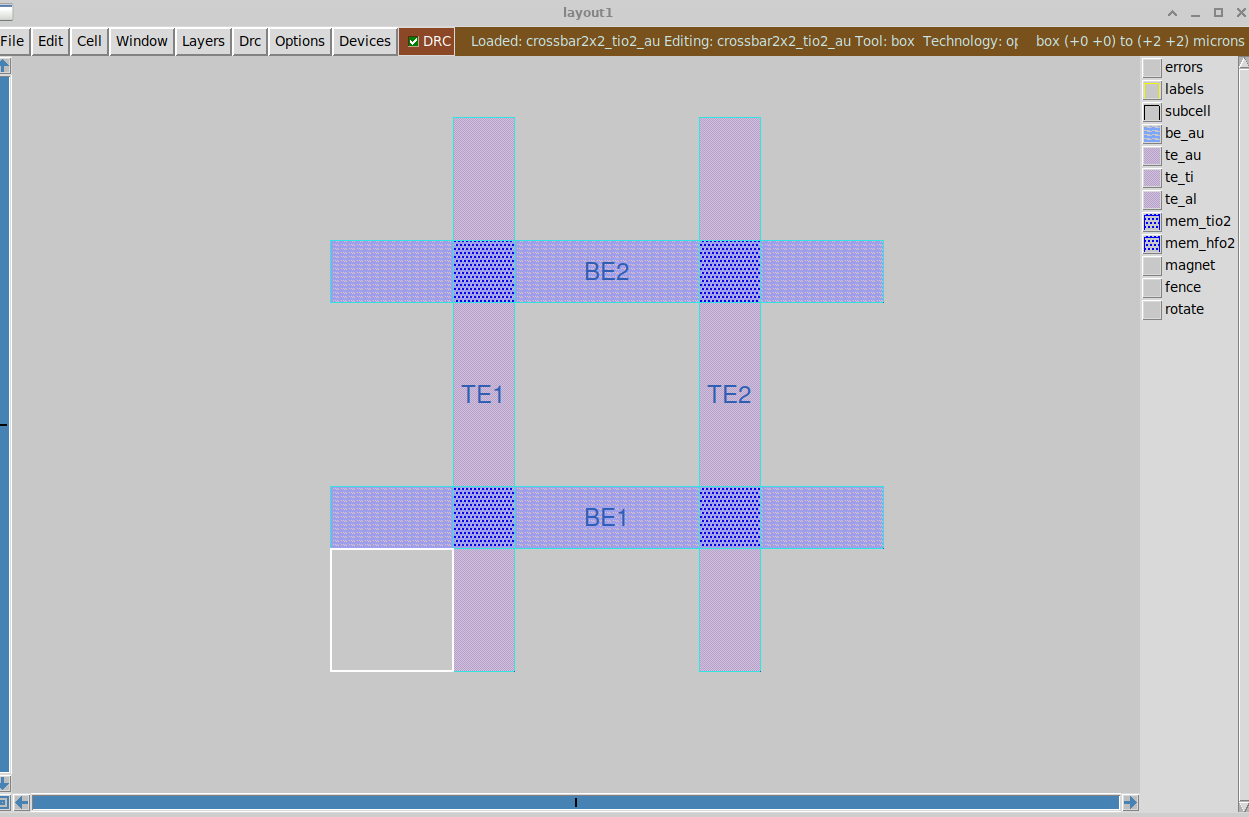
\includegraphics[width=0.55\textwidth]{figures/crossbar_magic_layout.png}
\end{center}
\footnotesize
Real, live Magic, \texttt{crossbar2x2\_tio2\_au} loaded -- the two
real \texttt{be\_au} rows (BE1/BE2) crossing the two real
\texttt{te\_au} columns (TE1/TE2), \texttt{mem\_tio2} visible as the
cross-hatched real overlap at each of the 4 real crosspoints.
\end{frame}

% ---------------------------------------------------------------
\begin{frame}[fragile]{Step 3 -- a real LEF macro}
A new \texttt{crossbar2x2\_tio2\_au} macro, appended to this
project's existing combined real LEF file:
\begin{center}
\begin{tabularx}{\textwidth}{lX}
\toprule
LEF field & Real value \\
\midrule
\texttt{SIZE} & 9.0 BY 9.0 (matches the real drawn footprint exactly) \\
\texttt{SYMMETRY} & X Y \\
Pins & \texttt{BE1}/\texttt{BE2}/\texttt{TE1}/\texttt{TE2}, each \texttt{DIRECTION INOUT}, \texttt{PORT} rect matching that row/column's own real position \\
\bottomrule
\end{tabularx}
\end{center}
\footnotesize
Real, live-verified: this project's own LEF parser reads the new macro
back correctly, and a no-edit re-export of the whole combined file
stays byte-identical for every macro this pass didn't touch.
\end{frame}

% ---------------------------------------------------------------
\begin{frame}{Step 4 -- the real Library Manager}
\begin{center}
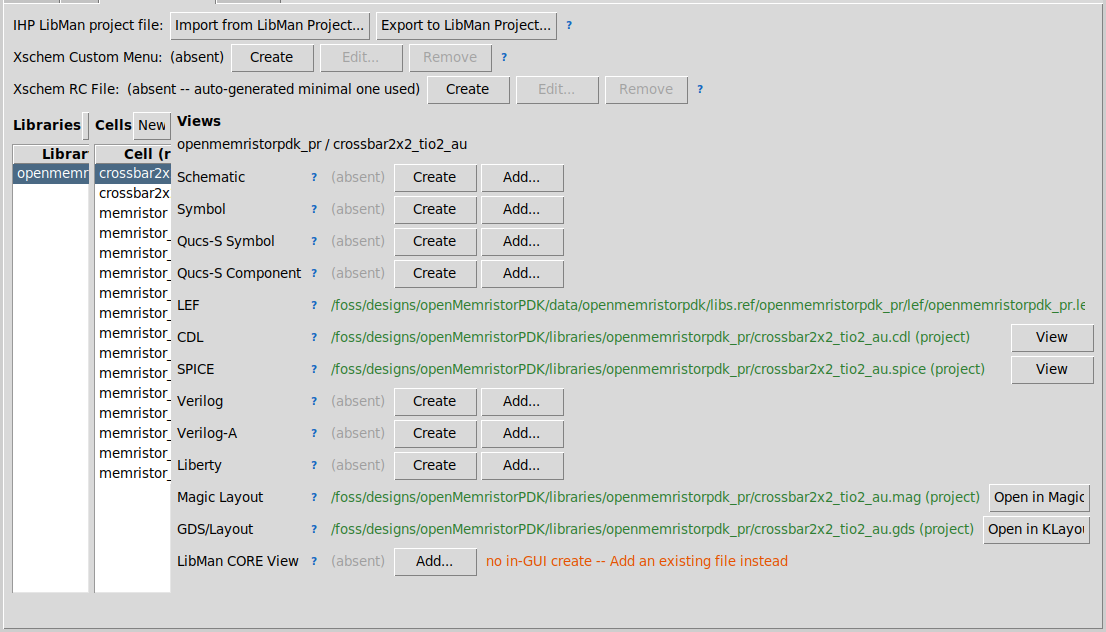
\includegraphics[width=0.65\textwidth]{figures/crossbar_library_manager.png}
\end{center}
\footnotesize
Real, live: the new cell, auto-discovered under
\texttt{openmemristorpdk\_pr} from its own real files (same stem,
\texttt{crossbar2x2\_tio2\_au}) -- real CDL/SPICE/Magic Layout/GDS
views all present, \textbf{Run LVS}/\textbf{Run DRC} both live.
\end{frame}

% ---------------------------------------------------------------
\begin{frame}{Step 5 -- real, live DRC}
\textbf{Run DRC} on the real Magic Layout view -- real GDS export,
then a real, live KLayout batch run against this project's own real
DRC deck (\texttt{BE.W.1}/\texttt{MEM1.W.1}/\texttt{MEM2.W.1}/\texttt{TE.S.1}):
\begin{center}
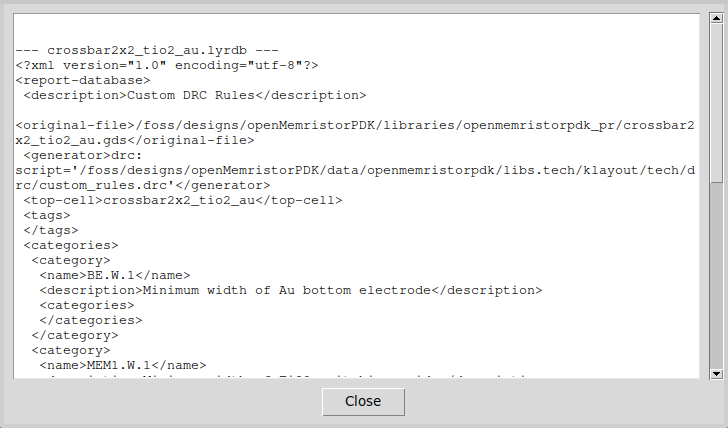
\includegraphics[width=0.65\textwidth]{figures/crossbar_drc_result.png}
\end{center}
\footnotesize
Real, live result: \textbf{0 violations} -- the real, generously-spaced
geometry from Step 1 pays off exactly as intended.
\end{frame}

% ---------------------------------------------------------------
\begin{frame}[fragile]{Step 6 -- real extraction, and a real, found limitation}
\textbf{Extract to SPICE} runs real Magic device-recognition
(\texttt{device subcircuit memristor\_tio2\_au\_prim be\_au te\_au},
this project's own existing \texttt{extract}-section line) against
the real layout. The real result:
\begin{cli}
.subckt crossbar2x2_tio2_au BE1 BE2 TE1 TE2
X0 BE2 tm_6_7# memristor_tio2_au_prim
X1 BE1 TE2 memristor_tio2_au_prim
.ends
\end{cli}
\footnotesize
Only \textbf{2} of the real 4 crosspoints, not 4 -- confirmed as a real
Magic limitation, not a layout bug, via several independent minimal
reproductions (down to one shared row, two separate columns) and
Magic's own real maintainer manual: \texttt{device subcircuit model
gate types [term types ...]} is built around a real transistor's own
gate/diffusion split, never designed for a flat, same-footprint
2-terminal device tapped multiple times onto one shared, undivided
bus.
\end{frame}

% ---------------------------------------------------------------
\begin{frame}[fragile]{Step 7 -- a real, hand-authored reference netlist}
Rather than reshape this real demo around that limitation, a real,
independent reference view describes the actually-intended topology
directly -- the same "hand-authored view of intended connectivity,
independent of the Magic Layout view" every other cell in this
project already has:
\begin{cli}
.SUBCKT crossbar2x2_tio2_au BE1 BE2 TE1 TE2
*.PININFO BE1:B BE2:B TE1:B TE2:B
X1 BE1 TE1 memristor_tio2_au_prim
X2 BE1 TE2 memristor_tio2_au_prim
X3 BE2 TE1 memristor_tio2_au_prim
X4 BE2 TE2 memristor_tio2_au_prim
.ENDS
\end{cli}
\footnotesize
This real, 4-device netlist is both the real LVS golden reference
(Step 8) and the real netlist Step 10's own simulation actually runs.
\end{frame}

% ---------------------------------------------------------------
\begin{frame}{Step 8 -- real, live LVS: an honest mismatch}
\textbf{Run LVS} -- real, live Netgen comparing the real, 2-device
extracted netlist (Step 6) against the real, 4-device reference (Step 7):
\begin{center}
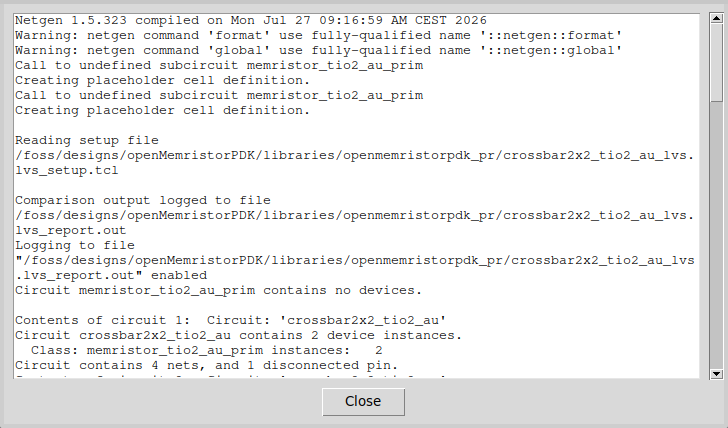
\includegraphics[width=0.65\textwidth]{figures/crossbar_lvs_result.png}
\end{center}
\footnotesize
Real, live, reported honestly: \texttt{Circuit crossbar2x2\_tio2\_au
contains 2 device instances} on the layout side, 4 on the reference
side -- a real mismatch, a direct, real, expected consequence of
Step 6's own finding, not silently papered over.
\end{frame}

% ---------------------------------------------------------------
\begin{frame}[fragile]{Step 9 -- designing the real write-then-read test}
A real, standard passive-crossbar bias: selected row $=V_w$, selected
column $=0$, every other row/column $=V_w/2$ -- writes just cell
(1,1), leaving (1,2)/(2,1) genuinely half-selected and (2,2) fully
untouched:
\begin{center}
\begin{tabularx}{\textwidth}{lXc}
\toprule
Phase & Real drive & Real effect \\
\midrule
Write (1,1) & BE1=1.0, TE1=0.0, BE2=TE2=0.5 & (1,1) full write; (1,2)/(2,1) real Vw/2 disturb; (2,2) untouched \\
Read row 1 & BE1=0.05, BE2=TE1=TE2=0 & I(TE1)=cell(1,1), I(TE2)=cell(1,2) \\
Read row 2 & BE2=0.05, BE1=TE1=TE2=0 & I(TE1)=cell(2,1), I(TE2)=cell(2,2) \\
\bottomrule
\end{tabularx}
\end{center}
\footnotesize
The real device model (HP linear ion-drift, Strukov et al. 2008) has
no real switching threshold -- any nonzero current drifts state, just
slower at half voltage, which made the real timing below genuinely
matter, not just the voltages.
\end{frame}

% ---------------------------------------------------------------
\begin{frame}{Step 9, continued -- two real bugs, found live}
\footnotesize
\begin{itemize}
  \item \textbf{The real unselect voltage must be exactly $V_w/2$.} A
        same-row/different-column cell sees $(V_w - V_{unsel})$; a
        same-column/different-row cell sees just $V_{unsel}$ -- those
        two real disturb voltages only match when $V_{unsel}=V_w/2$.
        An earlier pass tried a smaller, asymmetric 0.2V unselect
        voltage (hoping to slow the disturb further) and instead
        pushed one real disturb voltage up to 0.8V -- silently
        saturating a cell this deck means to show as merely disturbed.
  \item \textbf{Writing both diagonal cells doubles the off-diagonal
        disturb.} A first, two-write-phase version (also writing
        (2,2)) gave cells (1,2)/(2,1) a real, \emph{cumulative} 2x
        exposure to the unselect voltage -- enough to fully saturate
        them too, erasing the real gap. Fixed by writing only cell
        (1,1): every real cell now gets exactly one, honestly
        comparable exposure.
  \item Real duration tuning was done directly against the real,
        running OSDI model, not an idealized approximation -- an
        earlier, simplified Python reproduction of the model's own
        exact equation \emph{disagreed} with the real simulated
        trajectory and had to be abandoned.
\end{itemize}
\end{frame}

% ---------------------------------------------------------------
\begin{frame}{Step 10 -- the real, live result}
\begin{center}
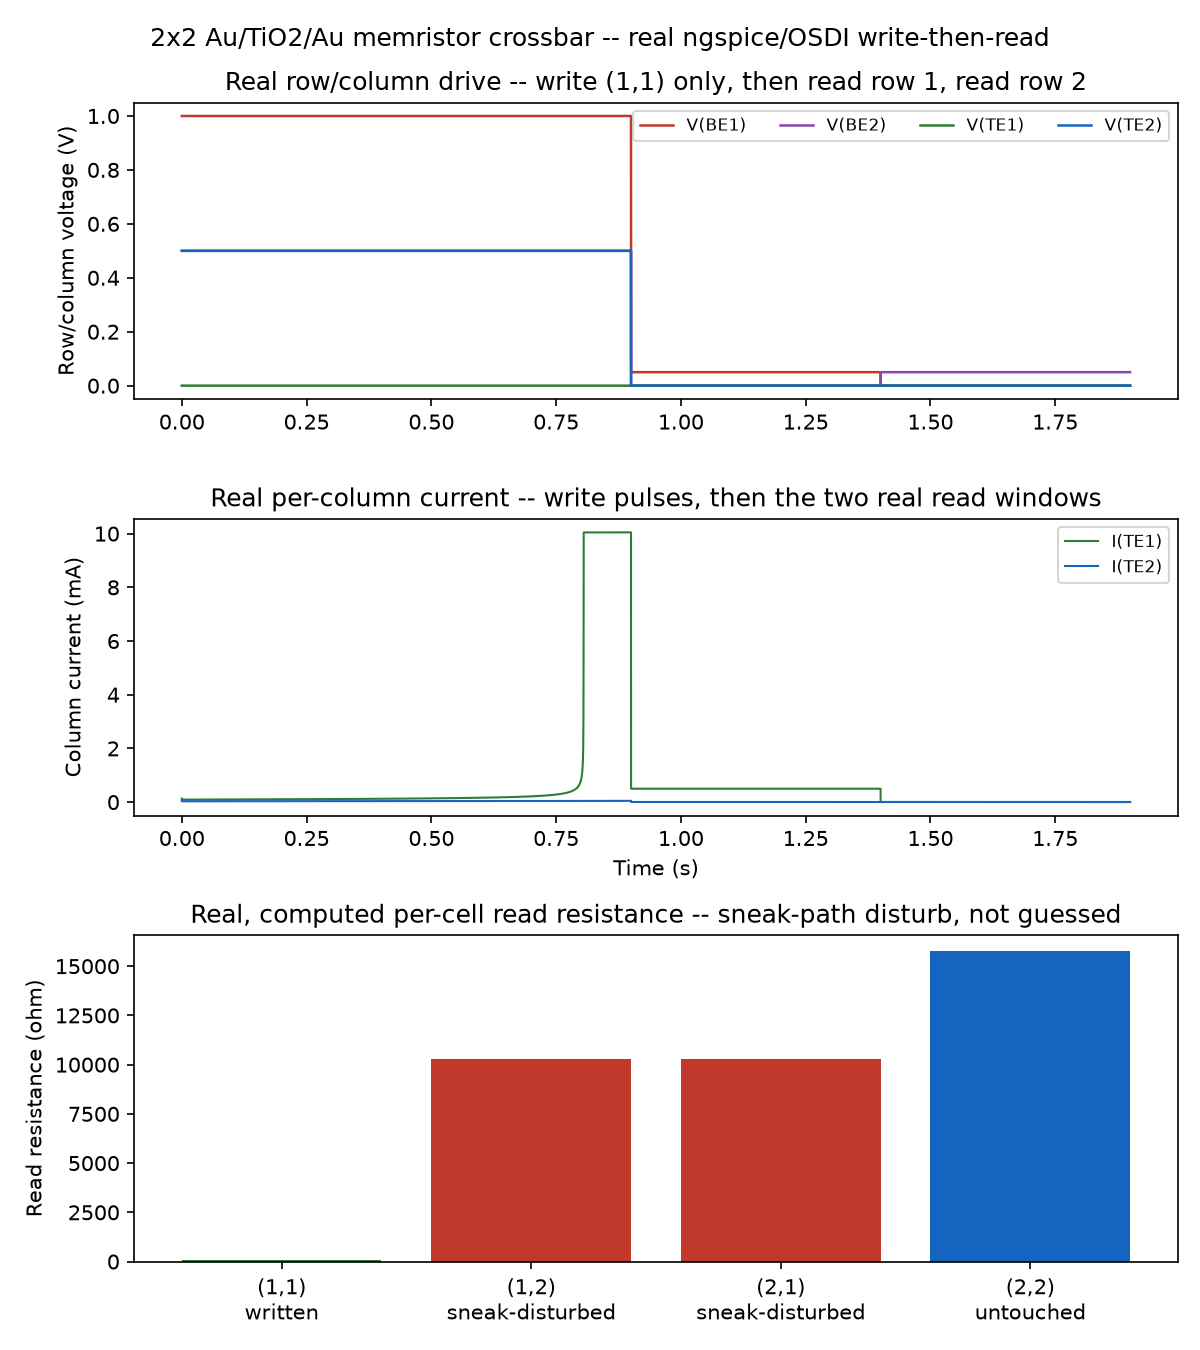
\includegraphics[width=0.5\textwidth]{figures/crossbar_write_read.png}
\end{center}
\footnotesize
Real, simulated (ngspice/OSDI): \textbf{100$\,\Omega$} (written) $\ll$
\textbf{10293$\,\Omega$} (sneak-disturbed) $<$ \textbf{15781$\,\Omega$}
(untouched) -- a clean, real, three-way contrast, not guessed.
\end{frame}

% ---------------------------------------------------------------
\begin{frame}{What this real example actually demonstrates}
\footnotesize
\begin{itemize}
  \item A full, real pipeline -- layout $\to$ LEF $\to$ extraction
        $\to$ LVS $\to$ DRC $\to$ simulation -- run against a genuine
        shared-bus crossbar topology, not four independent cells.
  \item A real, found tool limitation (Magic's own device-recognition
        model doesn't support a shared bus tapped by multiple
        2-terminal devices), characterized directly, not guessed, and
        worked around with a real, independent reference netlist
        rather than reshaping the demo to avoid it.
  \item A real, live-verified crossbar sneak-path disturb: writing one
        cell measurably, honestly perturbs its own real row/column
        neighbors, even though they were never themselves addressed --
        the concrete, real reason crossbar addressing needs real care,
        not just more density.
  \item Verified for real, driven: \texttt{tests/test\_crossbar2x2.py}
        -- real LEF/CDL parsing, a real 9x9um GDS export on the
        correct real GDS layers, the real 2-of-4 extraction limitation
        asserted explicitly, real LVS mismatch, real DRC clean.
\end{itemize}
\end{frame}

\end{document}
